\documentclass[tikz,border=4pt]{standalone}
\usepackage{pgfplots}
\usetikzlibrary{pgfplots.groupplots,calc}
\pgfplotsset{compat=1.18}

\definecolor{cprimary}{RGB}{147,190,227}
\definecolor{csecondary}{RGB}{229,154,145}
\definecolor{ctertiary}{RGB}{201,206,214}

\begin{document}
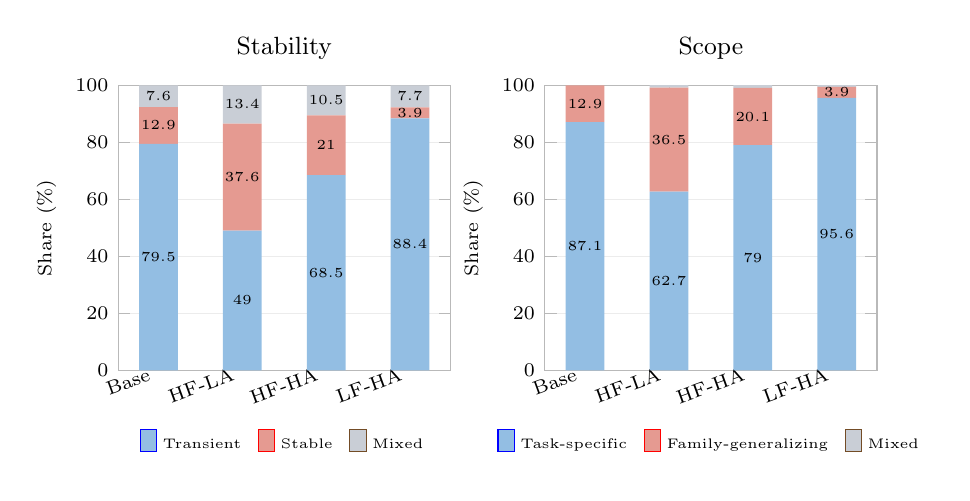
\begin{tikzpicture}
  \begin{groupplot}[
    group style={group size=2 by 1, horizontal sep=1.2cm},
    width=5.8cm,
    height=5.2cm,
    ymin=0,
    ymax=100,
    ybar stacked,
    symbolic x coords={Base,HF-LA,HF-HA,LF-HA},
    xtick=data,
    enlarge x limits=0.16,
    ylabel={Share (\%)},
    tick label style={font=\scriptsize},
    label style={font=\scriptsize},
    title style={font=\small},
    x tick label style={font=\scriptsize, rotate=20, anchor=east},
    ymajorgrids=true,
    grid style={draw=gray!15},
    axis line style={draw=gray!55},
    tick style={draw=gray!55},
    legend style={
      draw=none,
      fill=none,
      font=\tiny,
      legend columns=3,
      /tikz/every even column/.append style={column sep=4pt}
    },
    nodes near coords={\pgfmathprintnumber[fixed,precision=1]{\pgfplotspointmeta}},
    every node near coord/.append style={font=\tiny, text=black}
  ]
    \nextgroupplot[
      title={Stability},
      legend to name=stabilitylegend
    ]
      \addplot+[draw=none, fill=cprimary, bar width=14pt]
        coordinates {
          (Base,79.5)
          (HF-LA,49.0)
          (HF-HA,68.5)
          (LF-HA,88.4)
        };
      \addplot+[draw=none, fill=csecondary, bar width=14pt]
        coordinates {
          (Base,12.9)
          (HF-LA,37.6)
          (HF-HA,21.0)
          (LF-HA,3.9)
        };
      \addplot+[draw=none, fill=ctertiary, bar width=14pt]
        coordinates {
          (Base,7.6)
          (HF-LA,13.4)
          (HF-HA,10.5)
          (LF-HA,7.7)
        };
      \legend{Transient,Stable,Mixed}

    \nextgroupplot[
      title={Scope},
      legend to name=scopelegend
    ]
      \addplot+[draw=none, fill=cprimary, bar width=14pt]
        coordinates {
          (Base,87.1)
          (HF-LA,62.7)
          (HF-HA,79.0)
          (LF-HA,95.6)
        };
      \addplot+[draw=none, fill=csecondary, bar width=14pt]
        coordinates {
          (Base,12.9)
          (HF-LA,36.5)
          (HF-HA,20.1)
          (LF-HA,3.9)
        };
      \addplot+[draw=none, fill=ctertiary, bar width=14pt]
        coordinates {
          (Base,0.0)
          (HF-LA,0.9)
          (HF-HA,1.0)
          (LF-HA,0.6)
        };
      \legend{Task-specific,Family-generalizing,Mixed}
  \end{groupplot}

  \node[anchor=north] at ($(group c1r1.south)+(0,-0.55cm)$) {\pgfplotslegendfromname{stabilitylegend}};
  \node[anchor=north] at ($(group c2r1.south)+(0,-0.55cm)$) {\pgfplotslegendfromname{scopelegend}};
\end{tikzpicture}
\end{document}
